\documentclass[tikz]{standalone}
\usepackage{tikz,amsmath}
\usetikzlibrary{shapes}
\begin{document}
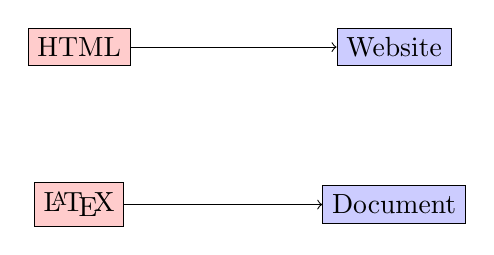
\begin{tikzpicture}
    \node (A) [rectangle, fill=red!20, draw] at (0, 0) {HTML};
    \node (B) [rectangle, fill=blue!20, draw] at (4, 0) {Website};
    \node (C) [rectangle, fill=red!20, draw] at (0, -2) {\LaTeX};
    \node (D) [rectangle, fill=blue!20, draw] at (4, -2) {Document};
    \draw [->] (A) -- (B);
    \draw [->] (C) -- (D);
\end{tikzpicture}
\end{document}
